\newpage
\pagestyle{empty}

\begin{minipage}[c]{.25\linewidth}
	
\includegraphics[width=4cm]{images/Logo-LEnsE.png}
\end{minipage} \hfill
\begin{minipage}[c]{.4\linewidth}

\begin{center}
\vspace{0.3cm}
{\Large \textsc{Opto-Electronique}}

\medskip

\textbf{\Large Ressources}

\end{center}
\end{minipage}\hfill

\vspace{0.5cm}

\noindent \rule{\linewidth}{1pt}
\section{Mesurer la bande-passante d'un système linéaire}
\label{ressource:BandePassante}


%%%%%%%%%%%%%%%%%%%%%%%%%%%%%%%%%%%%%%%%%%%%%%%%%%%%%%%%%%%%%%%%%%%%%%%%%%%%%%%%
%%%%%

La \textbf{bande-passante} est un \textbf{paramètre crucial} pour évaluer et concevoir des systèmes électroniques, des filtres, des amplificateurs et des circuits de communication. Elle est définie comme l'\textbf{intervalle de fréquences} pour lequel le système peut \textbf{transmettre des signaux avec une atténuation minimale}.

\medskip

Pour les systèmes linéaires et les filtres, la bande-passante est souvent mesurée entre les points où la puissance du signal de sortie est \textbf{réduite de $3\operatorname{dB}$} par rapport à la puissance du signal de sortie dans la bande-passante (voir figure~\ref{fig:rf_bp}).

\begin{figure}[h!]
    \centering
	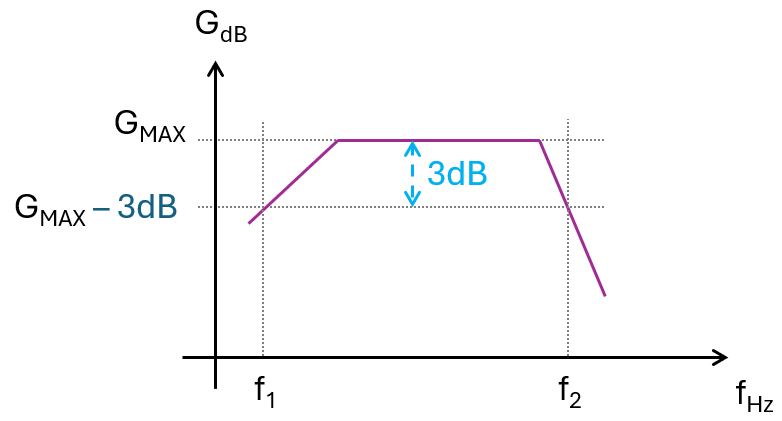
\includegraphics[width=0.6\textwidth]{images/bande_passante.png}
	
    \caption{Schéma de principe de la mesure de la bande-passante d'un système linéaire. Allure de la courbe de réponse en fréquence. La bande-passante de ce système s'étend de $f_1$ à $f_2$. Cela correspond donc à l'intervalle $\left[ f_1, f_2 \right]$.}
    \label{fig:rf_bp}
\end{figure}




\subsection{Mesure graphique}

A partir de la \textbf{réponse en fréquence}, il est possible de mesurer graphiquement la bande passante en cherchant le gain maximal du système et en regardant l'intersection des points passant par ce gain maximal réduit de $3\operatorname{dB}$ et l'axe des fréquences.


\subsection{Mesure expérimentale}

Cette réduction de $3\operatorname{dB}$ peut aussi être interprétée comme une \textbf{diminution de l'amplitude du signal d'un facteur} $\sqrt{2}$ par rapport à l'amplitude du signal de sortie dans la bande-passante (\textit{en supposant que le signal d'entrée reste constant en amplitude quelque soit sa fréquence}).

Il est donc possible de mesurer le gain maximal (à l'aide d'un oscilloscope ou d'un multimètre) en cherchant une fréquence telle que l'amplitude du signal de sortie sur celle d'entrée est maximale, en mesurant ces deux valeurs.

On cherche ensuite les amplitudes telles que le gain maximal est divisé par $\sqrt{2}$ et on relève les fréquences associées. Ces fréquences correspondent à la bande-passante.